% new tcolorbox environment
\newtcolorbox{headline}[2][]{
  coltext      = black,
  colframe     = \MyBlockFrameColorLeft,
  colback      = \MyBlockFillColorLeft,
  colbacktitle = \MyBlockTitleBoxColor,
  coltitle     = black,
  title        = {\Huge{\textbf{#2}}},
  fonttitle    = \bfseries,
  boxrule      = 0.2cm, %frame line width
  %tikz={rotate=#3}, % manipulate the tcolorbox as a whole (in degrees)
  top=+0.0cm, bottom=+0.0cm, left=+0.05cm, right=+0.05cm,
  %enlarge top by   = +1.0cm,  %  equivalent to mdframed 'skipabove'
  %enlarge bottom by= +0.0cm,  %  equivalent to mdframed 'skipbelow'
  %enlarge left by  = +1.5cm,  
  %enlarge right by = +0.0cm, 
  opacityback=1.0, % 1.0 means totally transparent, 0.0 means totally opaque
  arc=0.0cm,        % 0.0cm for non-rounded corners!
  #1,
}

% CMS
\begin{headline}[enhanced, tikz={rotate=0}]{Fotios Ptochos Promoted to Professor!}
  \begin{multicols}{2}
    \lipsum[1]\\ 
    \lipsum[2]\\ 
    %\lipsum[3]\\ 
    % ========================
    \begin{figure}
      \begin{center}
        \vspace{-0.2in}
        \leavevmode
        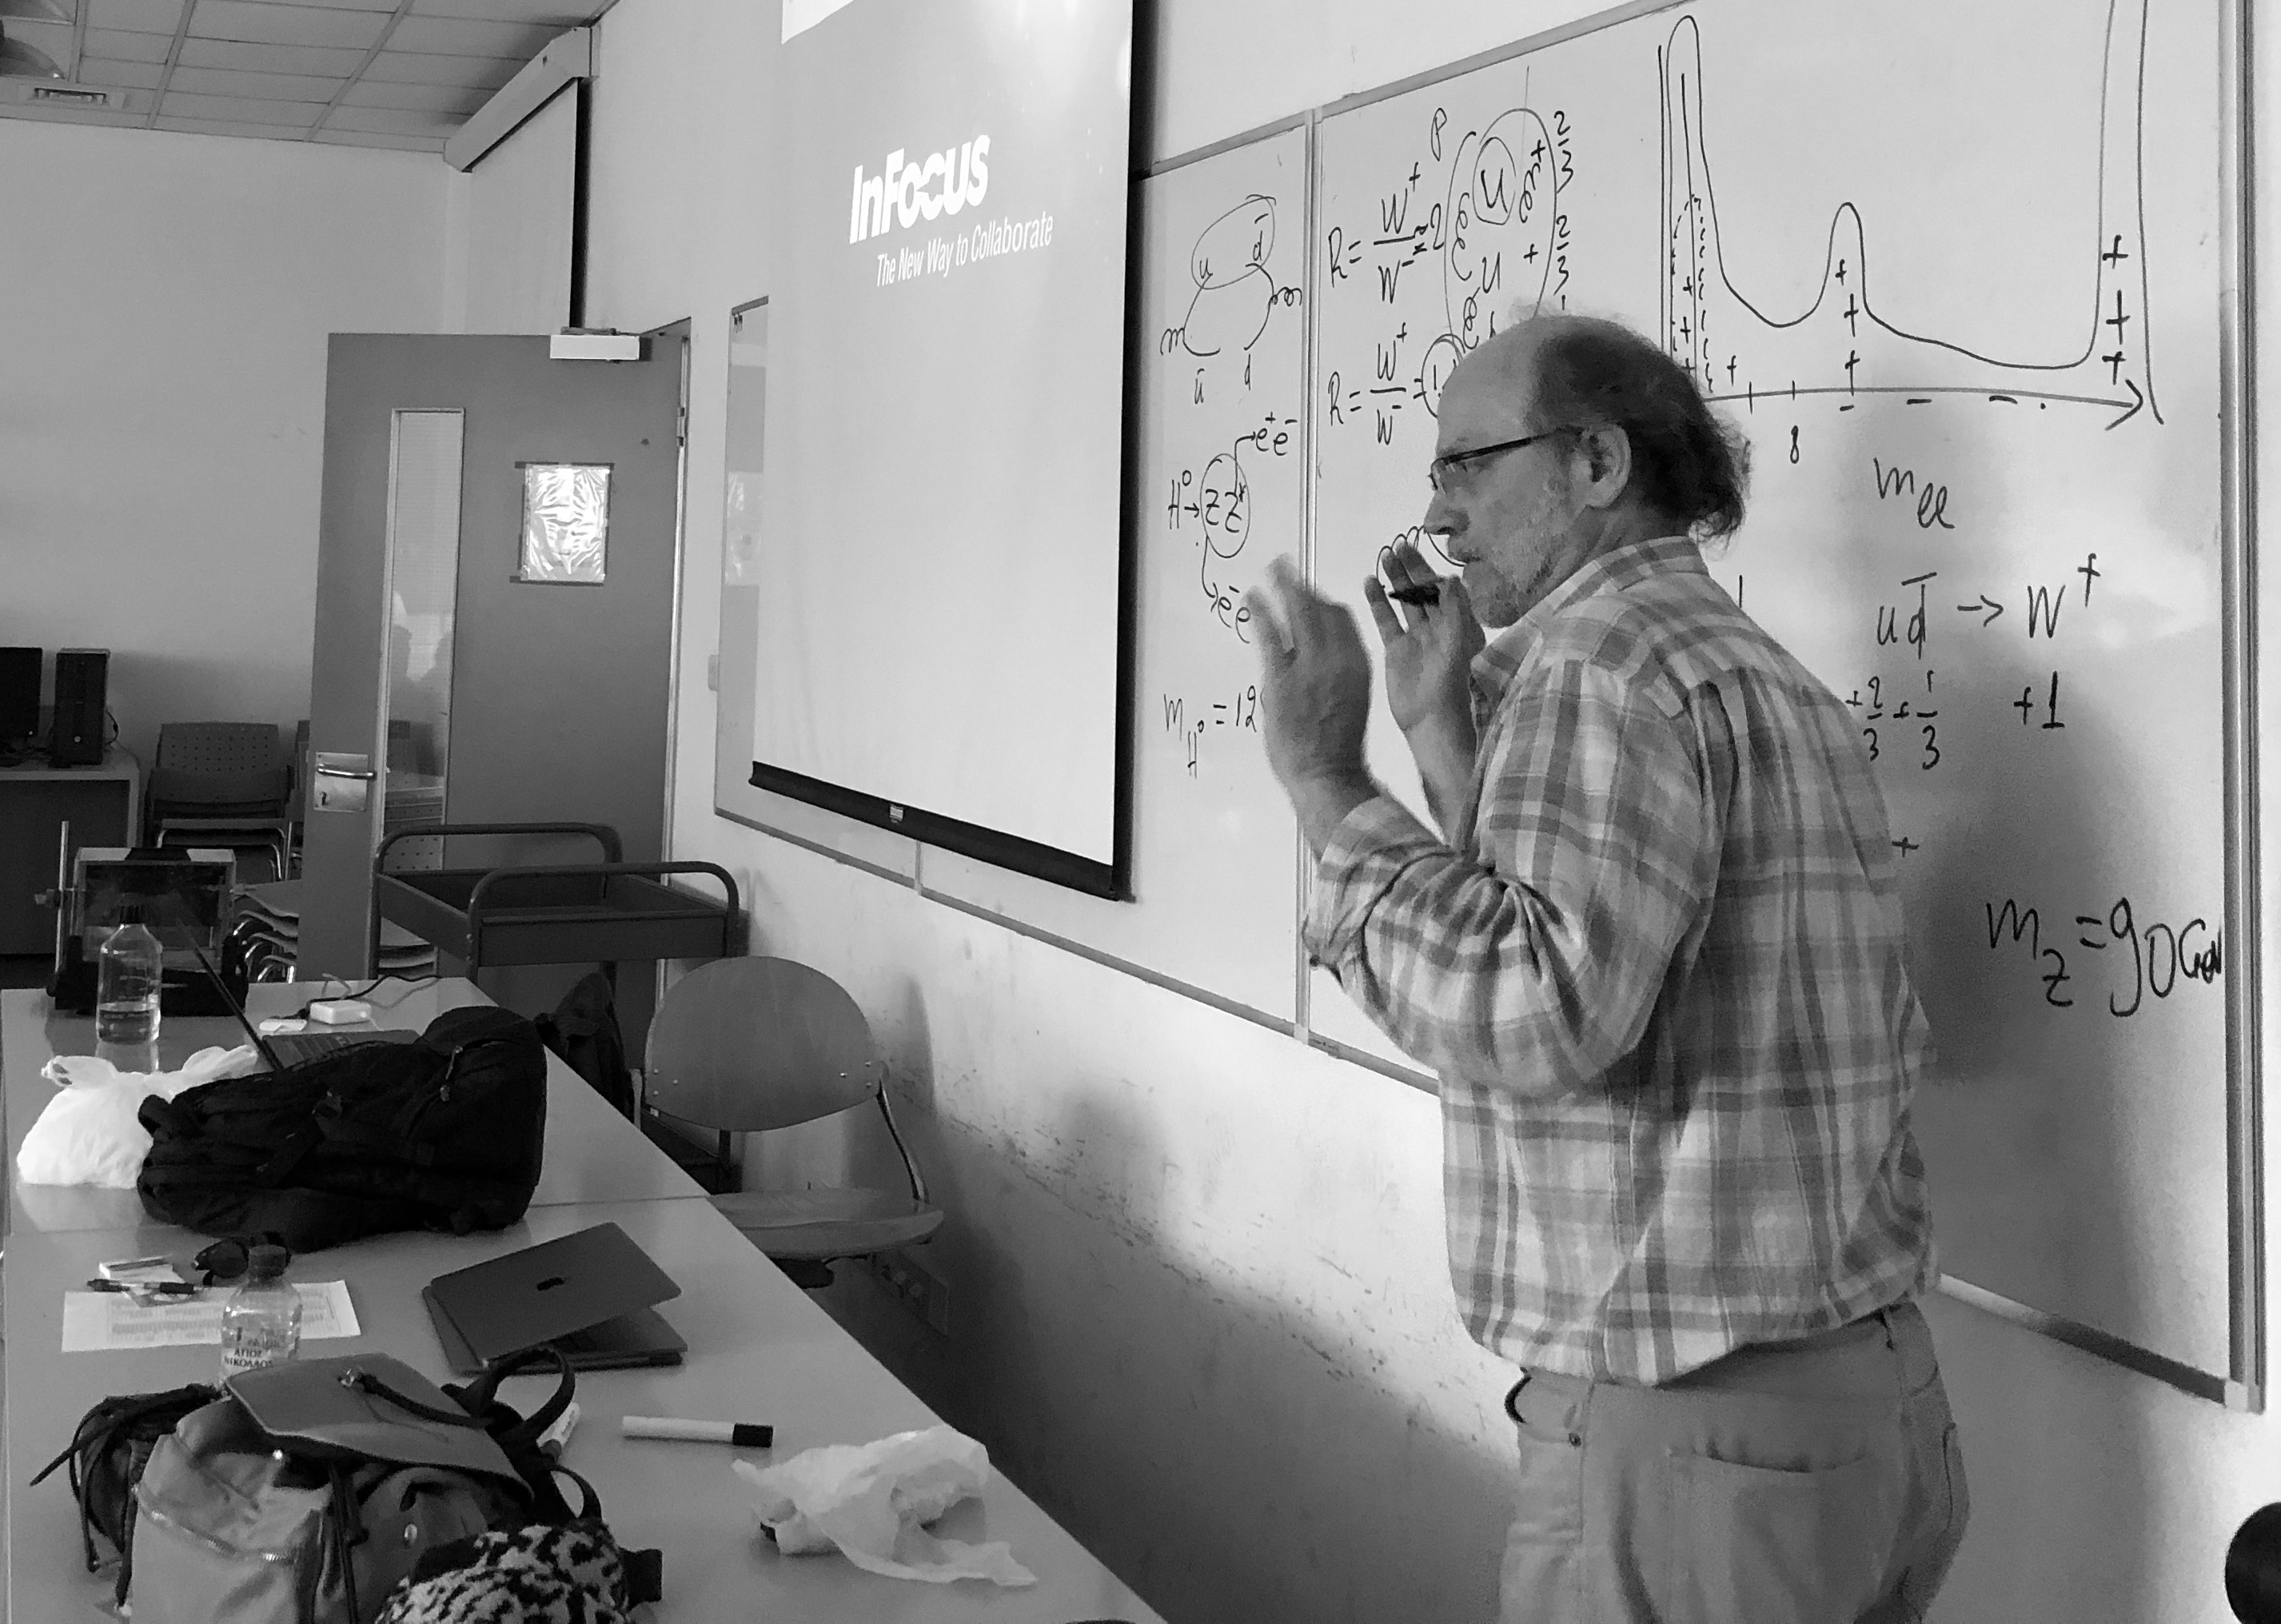
\includegraphics[width=0.5\textwidth]{./figures/Fotis6.png}
      \end{center}
    \end{figure}
    % ========================
  \end{multicols}
\end{headline}
